\subsubsection{System Linux, nagrywanie na pendriva}
\begin{wrapfigure}{r}{0.5\textwidth}
		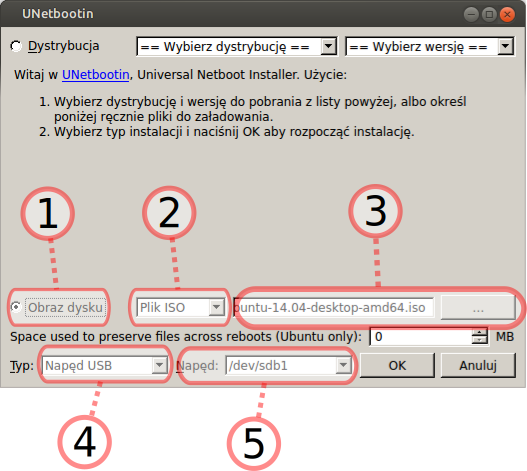
\includegraphics[width=\linewidth]{images/instalacja_nagrywanie_obrazu_linux.png}
\end{wrapfigure}
W systemach operacyjnych Linux do nagrywania obrazu na pendriva najlepiej posłużyć się programem UnetBootin, dostępnym w każdej dystrybucji. Podłącz do komputera napęd USB, który chcesz przeznaczyć na instalator Ubuntu.
\begin{enumerate}
\item Zaznacz pole Obraz dysku
\item Z menu wybierz Plik ISO
\item W to pole podaj ścierzkę do pobranego wcześniej obrazu instalatora Ubuntu. Wciśnij przycisk oznaczony trzema kropkami (\ldots) i wskaż plik.
\item W tym menu wybierz Napęd USB
\item Z tego menu wybierz podłączonego wcześniej pendriva.\\
\textbf{UWAGA: Wszystkie dane na nim zostaną skasowane!}
\item Kliknij przycisk OK aby rozpoczać nagrywanie
\end{enumerate}
\clearpage
\subsubsection{System Linux, nagrywanie na DVD}
%TODO potrzebny obrazek z włożoną płytą DVD i wybranym obrazem ubuntu 14.04
\begin{wrapfigure}{L}{0.5\textwidth}
		\includegraphics[width=\linewidth]{images/instalacja_nagrywanie_obrazu_linux_DVD.png}
\end{wrapfigure}
Aby nagrać obraz na płytę DVD potrzebujesz odpowiedniego programu. W tym przykładzie posłużymy się dostępną w większości dystrybucji nagrywarką Brasero. Kliknij prawym przyciskiem myszy na pobrany wcześniej obraz instalatora Ubuntu, wybierz Otwórz w a następnie Brasero. W otwartym oknie zostaniesz poproszony o włożenie czystej płyty DVD. Zrób to, a nastepnie kliknij na przycisk Nagraj.
\clearpage